%%%%%% CMB-S4 Simulations and Data Analysis Chapter, Implementation Section  %%%%%%%%%%%%%%%%
 
\section{Implementation Issues}

\subsection{Time-Ordered Data Volume \& High Performance Computing}

The quest for ever-fainter signals in the CMB drives us to gather ever-larger time-ordered data (TOD) sets to obtain the necessary signal-to-noise to uncover them. As Figure \ref{fig_cmb_hpc_scaling} shows, the volumes of ground-based, balloon-borne and satellite CMB data sets have exhibited exponential growth over the last 20 years and are anticipated to do so again over the next. Moreover, for suborbital experiments the exponent exactly matches that of Moore's Law for the growth of computing capability, where we us as a proxy here the peak performance of the flagship high performance computing (HPC) system at the DOE's National Energy Research Scientific Computing (NERSC) Center at any epoch (reflecting the widespread use of NERSC for CMB data analyses over the last 20 years). 

\begin{figure}[htbp]
\centering
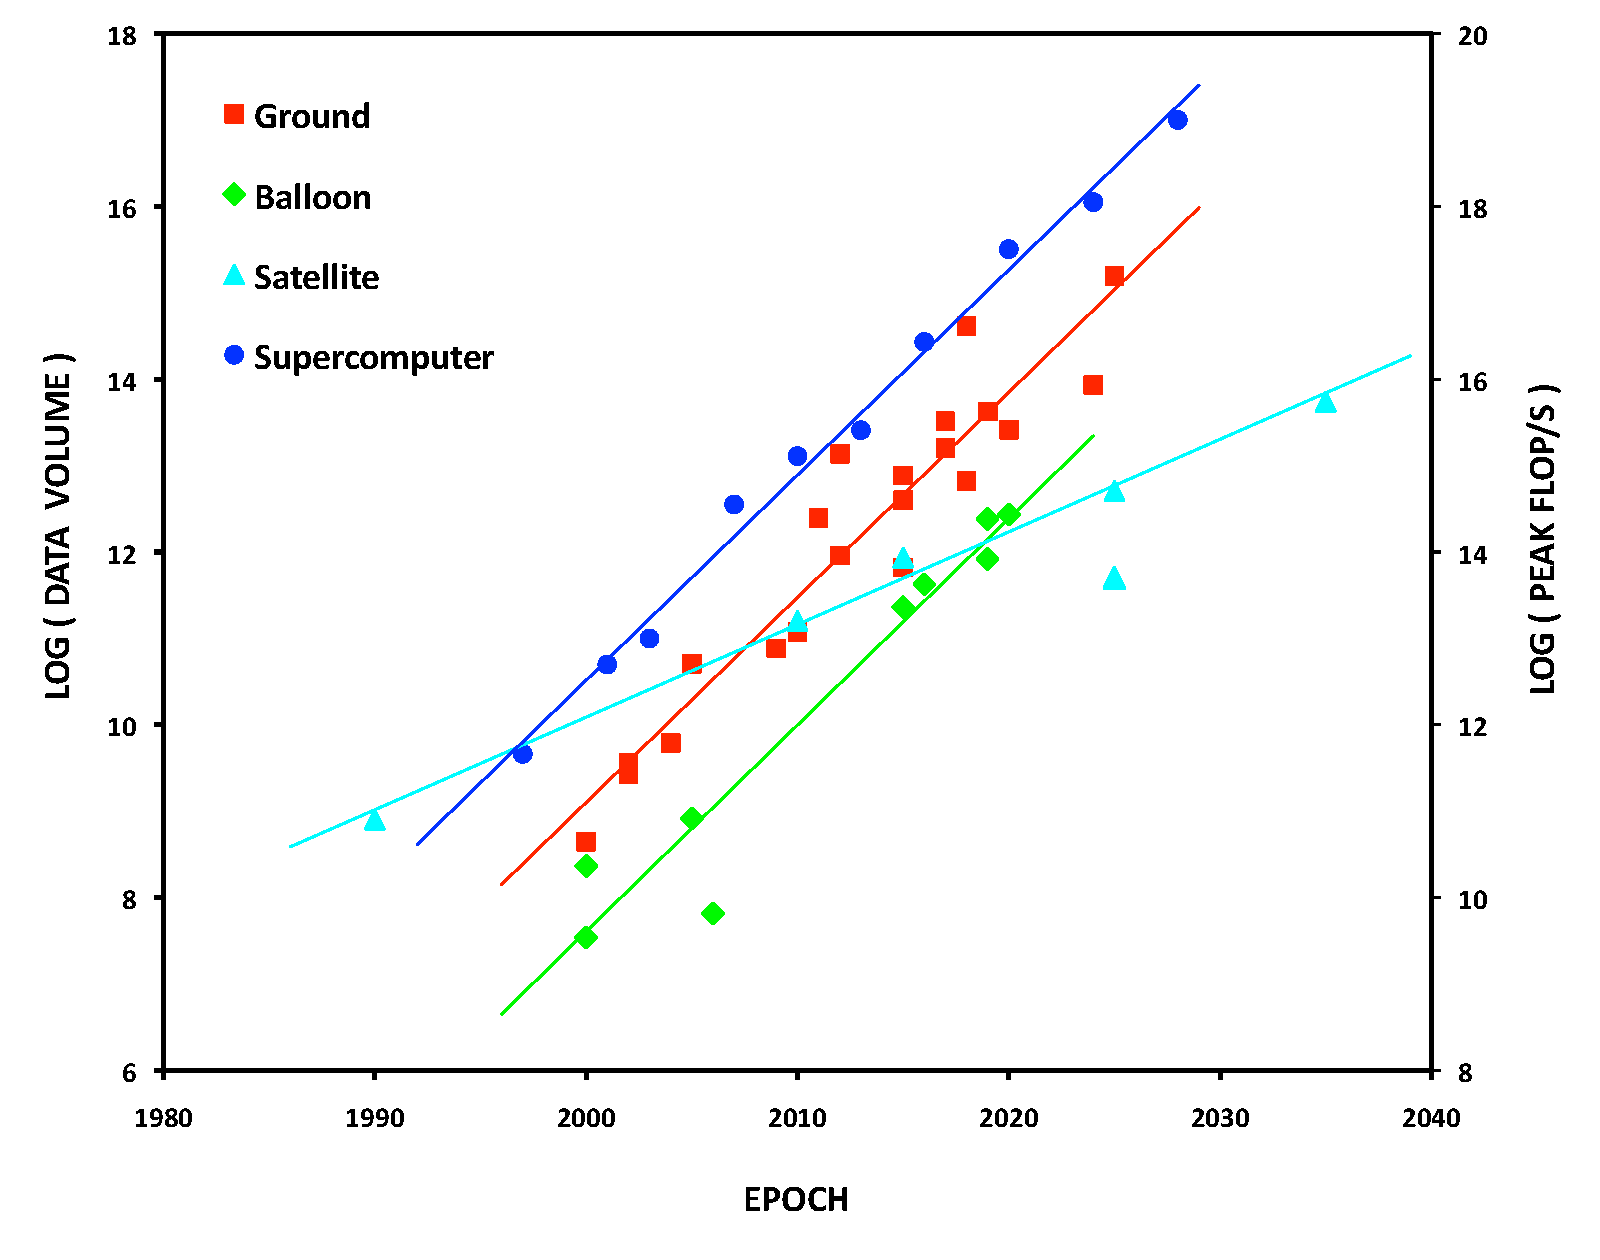
\includegraphics[width=0.5\textwidth]{Analysis/cmb_hpc_scaling}
\caption{Exponential growth of CMB time-ordered data volume and HPC capability: 1990 -- 2030.}
\label{fig_cmb_hpc_scaling}
\end{figure}

Furthermore, in the absence of a full covariance matrix we rely on Monte Carlo methods for uncertainty quantification and debiasing, and to achieve the desired percent-level statistical uncertainty requires us to simulate and reduce $10^4$ realizations of the data. Taken together, this implies that all TOD-processing steps (in simulation or analysis) must employ algorithms that scale no worse than linearly in the number of samples, and that these algorithms must then be implemented efficiently on the largest high performance computing (HPC) platforms available to us. 

The most massive Monte Carlo sets generated to date have been the Full Focal Plane (FFP) sets in support of the analysis of the Planck satellite data, with FFP8 comprising $10^4$ realizations of the mission reduced to O($10^6$) maps. Key to achieving this scale has been an aggressive optimization of the software stack, coupled with system-specific tuning over 6 generations of NERSC supercomputer. In particular wherever possible TOD input/output (IO) is removed from the pipeline so that, for example, instead of pre-computing the TOD and then pre-processing/mapping it, each realization is generated on demand and passed to the analysis pipeline in memory. While this necessitates the re-simulation of a realization should further analysis be required, it is still very substantially faster than writing it to disk and reading it back in. Similarly, inter-process communication is optimized by using a hybridized MPI/OpenMP implementation that employs explicit message passsing for inter-node, and threading for intra-node, communication.

A critical challenge for CMB-S4 will be to preserve this capability on the coming generations of HPC architectures. 


\subsection{Application Interfaces, Data Objects and Formats}

%\bibliography{cmbs4}

%%
%% Populate the .bib file with entries from SPIRES Bibtex (preferred)
%% or ADS Bibtex (if no SPIRES entry).
%%  SPIRES will also supply the CITATION line information; please include it.
%%


